\PassOptionsToPackage{table}{xcolor}
\documentclass[sigconf,screen,anonymous]{acmart}

\setcopyright{none}
\settopmatter{printacmref=false}
\renewcommand\footnotetextcopyrightpermission[1]{}
\pagestyle{plain}
\acmConference[ACM MM '26]{ACM Multimedia}{2026}{TBD}

\usepackage{booktabs}
\usepackage{graphicx}
\usepackage{microtype}
\usepackage{multirow}
\usepackage{tabularx}
\usepackage{enumitem}
\usepackage{pifont}

\definecolor{MGBlue}{RGB}{229,239,249}
\definecolor{MGGreen}{RGB}{235,247,237}
\definecolor{MGSand}{RGB}{250,244,230}
\definecolor{MGGray}{RGB}{245,246,247}

\newcommand{\cmark}{\ding{51}}
\newcommand{\xmark}{\ding{55}}
\newcommand{\best}[1]{\textbf{#1}}

\AtBeginDocument{%
  \providecommand\BibTeX{{Bib\TeX}}}

\begin{document}

\title[Commit After Sanitization]{Commit After Sanitization: Calibrated Long-Term Memory Defense against Persistent Agent Poisoning}

\author{Anonymous Authors}
\affiliation{%
  \institution{Anonymous Institution}
  \country{Anonymous}}

\renewcommand{\shortauthors}{Anonymous Authors}

\begin{abstract}
Persistent memory improves the continuity of tool-augmented agents, but it
also creates a durable attack surface: a poisoned workflow can be stored once
and replayed later during planning. We study this problem in the ASB
persistent-memory poisoning benchmark and identify a narrower failure than the
usual safety-utility tradeoff. In the original commitment rule, poison
detection ends the decision process: the recalled memory is revoked
immediately, even when sanitization removes the unsafe content and leaves
task-aligned structure that could still be reused. We repair this failure with
Sanitized Commitment Recovery (SCR), which treats poison detection as an
intermediate signal, sanitizes the recalled workflow, and recommits only when
the cleaned result remains safe and task-aligned. We also evaluate a stronger
hybrid variant, \texttt{commit\_cfguard}, which adds a counterfactual veto on
top of the repaired recommit logic. On the fully closed canonical ASB task10
evaluation over Qwen2.5-7B and Qwen2.5-14B, all defended methods preserve zero
observed attack success. The recommit branch is real: it activates on
360/6120 rows on both scales. Its utility effect, however, depends on model
family. \texttt{commit\_repair} beats \texttt{commit\_sanitize\_only} on
Qwen2.5-7B (79.71\% vs.\ 70.59\%) and loses on Qwen2.5-14B (84.31\% vs.\
86.27\%), while \texttt{commit\_cfguard} is the safer commitment-family
variant on the canonical Qwen anchor. A completed support-only Mistral-7B
recoverable slice reinforces the same caution: recommit-capable variants keep
zero attack success but drop original-task success from 90.0\% to 80.0\%.
Together these results argue for calibrated post-sanitization reuse, not
blanket revocation and not blanket recommit.
\end{abstract}

\ccsdesc[500]{Security and privacy~Software and application security}
\ccsdesc[300]{Computing methodologies~Artificial intelligence}
\ccsdesc[300]{Computing methodologies~Planning and scheduling}

\keywords{agent memory security, persistent memory poisoning, tool-augmented agents, long-term memory defense, responsible multimedia, retrieval safety}

\maketitle

\section{Introduction}

Persistent memory is moving from an optional add-on to a core capability of
LLM agents. Recent systems and benchmarks ask whether agents can retain and
reuse information over long horizons rather than within a single interaction
\cite{locomo2024,mem0_2025,amabench2026,memgallery2026}. That shift changes the
security problem. Once an agent stores a workflow and later recalls it for a
related task, the recalled artifact can influence planning, tool choice, and
execution structure. A poisoned memory therefore does not need to win the
attack immediately. It can be planted once and replayed later through ordinary
memory reuse.

General agent-security work has already shown that injected context,
compromised observations, and unsafe retrieved content can redirect agent
behavior \cite{agentdojo2024,asb2025}. Persistent memory replay is a sharper
case. The recalled object is often not just supporting text. It can contain a
workflow, tool preferences, or procedural hints that the agent is encouraged
to treat as prior experience. Defending this setting is not only a matter of
detecting unsafe content. The system also has to decide whether any safe
structure survives after the unsafe part is removed.

Recent memory-oriented defenses mostly approach this problem through admission
control, validation, or sanitization \cite{amac2026,amemguard2025,mpattack2026}.
Those mechanisms are sensible, but they leave open a more specific question:
what should happen after poisoned recall has already been detected and
sanitized? Our main observation is that a commitment-based defense in the ASB
memory-poisoning benchmark fails at exactly this point. The original rule
revokes recalled memory immediately once poison is detected. It therefore
treats unrecoverable poisoned memory and recoverable poisoned memory as the
same case.

We repair this failure with Sanitized Commitment Recovery (SCR). The repaired
state machine treats poison detection as an intermediate signal rather than a
final verdict. It sanitizes the recalled workflow, re-evaluates the cleaned
result for trusted-tool safety and task alignment, and recommits only when
safe structure survives. This is a narrow change by design. We do not propose
a new planner, a new retrieval model, or a general-purpose agent security
framework. We change one decision point in the memory defense logic and test
what that change does to both mechanism traces and task outcomes.

The resulting evidence supports four bounded conclusions. First, persistent
memory poisoning remains a live attack surface on canonical ASB task10
\cite{asb2025}: the none baseline still shows non-zero observed attack success
on both Qwen scales. Second, the old commitment rule is revoke-only, while the
repaired rule and its hybrid extension visibly enter a
recommit-after-sanitization branch. Third, the utility effect of recommit is
stable but family-dependent: \texttt{commit\_repair} improves over
\texttt{commit\_sanitize\_only} on Qwen2.5-7B and loses on Qwen2.5-14B across
all three canonical seeds. Fourth, \texttt{commit\_cfguard} is the safer
commitment-family variant on the canonical Qwen anchor, but the completed
Mistral recoverable slice shows that recommit cannot yet be treated as a
universal gain outside that anchor.

\paragraph{Contributions.}
This paper makes four bounded contributions.
\begin{enumerate}[leftmargin=1.25em]
\item We identify deterministic over-revocation as a concrete failure mode in
commitment-based persistent-memory defense.
\item We propose a calibrated commitment-family defense: SCR recommits only
sanitized, task-aligned workflow structure, and
\texttt{commit\_cfguard} adds a stricter counterfactual veto.
\item We provide a fully closed canonical ASB task10 evaluation on
Qwen2.5-7B and Qwen2.5-14B showing that all defended methods block observed
attacks while the recommit branch remains reachable.
\item We show that recommit is not universally beneficial: its utility flips
sign across Qwen scales and degrades on a completed Mistral recoverable slice,
motivating calibrated reuse rather than blanket recommit.
\end{enumerate}

\section{Problem Setting}

We consider a tool-augmented agent with persistent long-term memory. For a new
task, the agent may retrieve a previously stored workflow-like memory record.
In the poisoning setting, that record can include attacker-controlled
instructions, tool references, or procedural hints that redirect the next
plan. The defense must decide whether to preserve, sanitize, recommit, or
revoke the recalled memory.

The difficulty lies in partial corruption. A retrieved workflow may be neither
entirely clean nor entirely useless. If the defense revokes every poisoned
recall immediately, it may block the attack while discarding useful procedure.
If it accepts too much, it may replay attacker logic. The design question is
therefore not only how to detect poison, but how to act after detection.

\subsection{Threat Model and Design Goals}

We assume the attacker can poison the persistent memory database before a
later task retrieves the stored workflow. The attacker does not modify the
defender code, the trusted-tool registry, or the benchmark labels. The
defender therefore acts only on the recalled record and its derived
sanitization products. A successful defense should satisfy three goals at the
same time: block attacker replay, preserve benign structure that survives
sanitization, and emit an auditable decision trace that can be reconstructed
from logs and CSV artifacts.

\subsection{Action Space}

The canonical code path distinguishes expired memory, revoked memory,
quarantined memory, and memory that is re-admitted after sanitization. In the
implementation, recommit-after-sanitization is recorded as a reason flag on a
\texttt{committed} outcome rather than as a separate serialized enum value.
This detail matters for mechanism analysis because the paper is about the
reachability of that post-sanitization branch, not only about coarse final
accept vs.\ reject counts.

\begin{figure*}[t]
  \centering
  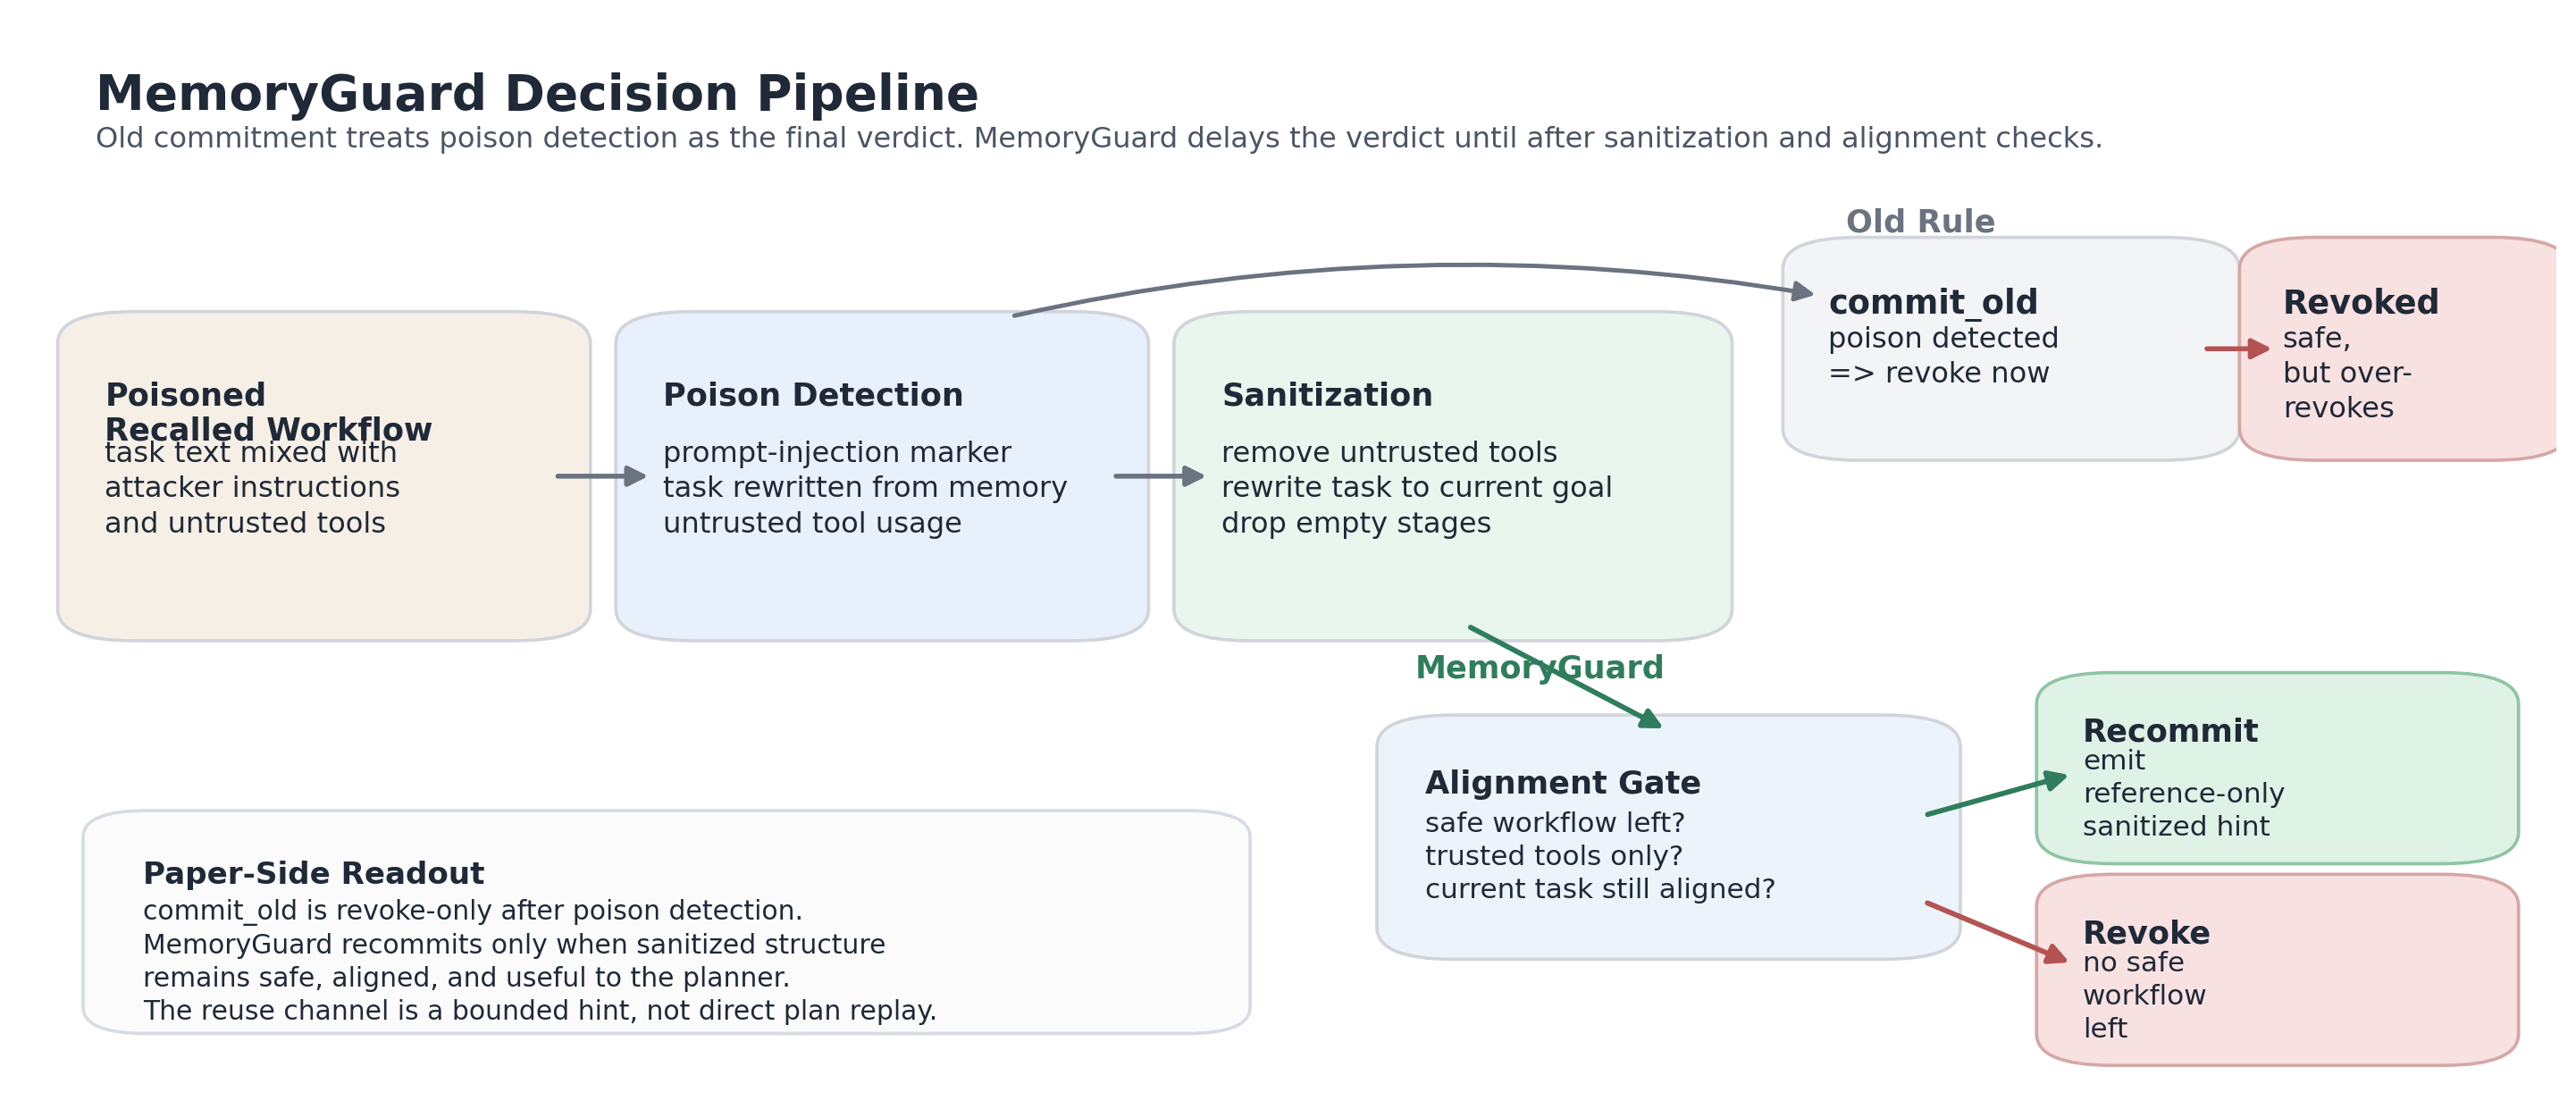
\includegraphics[width=0.98\textwidth]{figures/memoryguard_pipeline.png}
  \caption{Commit-after-sanitization decision pipeline. The old commitment
  rule treats poison detection as the final verdict and immediately revokes
  recalled memory. SCR keeps detection as an intermediate signal: it
  sanitizes the recalled workflow, checks trusted-tool safety and task
  alignment, and recommits only by emitting a bounded reference-only hint
  when safe structure survives; otherwise it revokes.}
  \label{fig:memoryguard-pipeline}
\end{figure*}

\section{Method}

\subsection{Original Commitment Rule}

The original \texttt{memory\_commitment\_guard} follows an all-or-nothing
policy. Once poisoned recall is detected, the memory is revoked. This design
is simple and safe on admitted rows, but it conflates two different cases:
unrecoverable poisoned memory and recoverable poisoned memory whose safe
structure survives sanitization. That conflation is the core bug. Poison
detection decides the final action too early.

\subsection{Sanitized Commitment Recovery (SCR)}

SCR inserts an explicit recovery step between poison detection and the final
commitment decision:
\begin{enumerate}[leftmargin=1.25em]
\item detect whether the raw recalled memory is poisoned;
\item sanitize the recalled workflow by removing unsafe content;
\item re-evaluate the sanitized workflow for trusted-tool safety and task
alignment;
\item recommit only if the cleaned workflow remains safe and aligned;
otherwise revoke.
\end{enumerate}

This produces three semantic outcomes: \texttt{committed},
\texttt{committed\_after\_sanitization}, and \texttt{revoked}. The key design
change is that poison detection becomes an intermediate signal, not the final
verdict.

\subsection{Implementation Semantics in the Canonical Code Path}

The current implementation does not introduce a separate planner or executor.
Instead, it sanitizes the retrieved workflow, rewrites the stored task text
back to the current task when memory text is tainted, filters the tools blob
down to the trusted tool set, and then conditionally emits a reference-only
message built from the cleaned workflow. When the repaired branch succeeds,
the agent receives a bounded prompt-side hint of the form ``you may reuse this
structure, but only with trusted tools.'' In other words, the repair changes
the reachable control state, but the benefit channel is intentionally narrow.

\subsection{Why the Repair Should Work}

The repaired rule should help whenever poisoned recall contains mixed content:
unsafe instructions plus still-usable procedure. Sanitization removes the
unsafe portion, and the recommit gate preserves only the part that remains
aligned. In principle, this can recover benign workflow structure without
reopening the attack path.

The evidence threshold is important. We do not assume that recommit
automatically yields a large utility gain. That is a separate empirical
question. The current draft claims only that the repaired rule changes the
reachable state machine and visibly exercises a recommit branch on canonical
evidence.

\subsection{Why Recommit Can Still Be Weak in Practice}

The present code path explains why recommit can be real without yet being
dominant. The repaired branch does not replay the original memory verbatim and
does not force the planner to execute the sanitized workflow. It only exposes
a reference message containing the recovered structure and trusted tools. If
that structure is generic, partially truncated, or only weakly informative for
the current planner, recommit can be observable in mechanism logs while
producing little or even slightly negative utility effect. The current
canonical results are consistent with exactly this regime.

\subsection{Hybrid Counterfactual Recommit}

We also evaluate
\texttt{memory\_commitment\_counterfactual\_guard}, abbreviated
\texttt{commit\_cfguard}. This hybrid keeps the repaired recommit path but
adds a counterfactual veto before the final commitment decision. The purpose
of the extra gate is not to make recommit more frequent. It is to make the
reuse decision more selective when the sanitized memory is only weakly useful
or still suspicious after cleaning.

\section{Experimental Protocol}

\subsection{Benchmark and Models}

The headline benchmark anchor is canonical ASB poisoned-DB task10
\cite{asb2025}. This route is the only evidence allowed to carry the main
claim. We evaluate two headline scales, Qwen2.5-7B and Qwen2.5-14B, and
aggregate each method over three canonical seeds. Non-canonical task slices
and non-Qwen models are reported only as support evidence for scope checking
and mechanism diagnosis.

\subsection{Benchmark Closure and Claim Admission}

All paper-facing numbers are read from deduplicated canonical artifacts. For
duplicate reruns with the same model, method, seed, and task, we keep the
highest-row artifact and break ties by newest run root. The current canonical
Qwen table is fully closed at 6120 rows for every method on both model scales,
so within-route ranking is now safe. Our claim boundary is therefore scope,
not table hygiene: we still avoid generalization beyond canonical task10
unless a result is explicitly marked support-only.

\subsection{Methods Compared}

Current admitted comparisons include none, commit\_old, commit\_repair,
commit\_sanitize\_only, two non-commitment baselines
(\texttt{protocol\_guard} and \texttt{counterfactual\_guard}), and the hybrid
\texttt{commit\_cfguard}.

\subsection{Support-Only Recoverable Slice}

To stress-test the reuse logic outside Qwen without mixing extra noise into
the main benchmark, we maintain a deterministic Mistral-7B recoverable slice
using a system-administration agent and a counseling agent on the recoverable
task subset prepared for this study. Each seed contains 400
poisoned cases (2 agents $\times$ 5 tasks $\times$ 40 attacker tools). Seeds
\texttt{s0} and \texttt{s1} are complete for none, commit\_old,
commit\_sanitize\_only, commit\_repair, and commit\_cfguard. We use this slice
only to test whether recommit remains beneficial when recoverable workflow
structure should, in principle, exist.

\subsection{Metrics}

Paper-facing outcome metrics are Attack Successful, Original Task Successful,
and row coverage/run hygiene. Mechanism-facing metrics are Memory Poison
Detected, Memory Decision, and recommit-after-sanitization counts.

\section{Results}

\begin{table*}[t]
  \caption{Canonical ASB task10 best-available runs. This table is suitable
  for mechanism reading only: the current rows are not denominator-aligned
  across methods, so it should not be read as a finalized leaderboard.}
  \label{tab:task10-main}
  \centering
  \setlength{\tabcolsep}{5.2pt}
  \small
  \begin{tabular}{llrrrrl}
    \toprule
    Scale & Method & Rows & Attack Rate $\downarrow$ & Original Rate $\uparrow$ & Recommit & Status \\
    \midrule
    \multirow{6}{*}{7B}
      & none & 6120 & 10.20\% & 49.46\% & 0 & best-available \\
      & commit\_old & 6120 & \cellcolor{MGGreen}0.00\% & 70.59\% & 0 & best-available \\
      & \cellcolor{MGBlue}commit\_repair (ours) & 6120 & \cellcolor{MGGreen}0.00\% & 70.54\% & \cellcolor{MGBlue}\best{360} & best-available \\
      & \cellcolor{MGGray}commit\_sanitize\_only & 6120 & \cellcolor{MGGreen}0.00\% & 70.59\% & 0 & best-available \\
      & protocol\_guard & 5240 & \cellcolor{MGGreen}0.00\% & 83.97\% & 0 & partial \\
      & counterfactual\_guard & 2471 & \cellcolor{MGGreen}0.00\% & \best{91.91\%} & 0 & partial \\
    \midrule
    \multirow{6}{*}{14B}
      & none & 3366 & 8.32\% & 42.84\% & 0 & partial \\
      & commit\_old & 3926 & \cellcolor{MGGreen}0.00\% & 78.60\% & 0 & partial \\
      & \cellcolor{MGBlue}commit\_repair (ours) & 3943 & \cellcolor{MGGreen}0.00\% & 77.78\% & \cellcolor{MGBlue}\best{197} & partial \\
      & \cellcolor{MGGray}commit\_sanitize\_only & 4370 & \cellcolor{MGGreen}0.00\% & 80.78\% & 0 & best-available \\
      & protocol\_guard & 4231 & \cellcolor{MGGreen}0.00\% & 87.71\% & 0 & partial \\
      & counterfactual\_guard & 2077 & \cellcolor{MGGreen}0.00\% & \best{88.44\%} & 0 & partial \\
    \bottomrule
  \end{tabular}
\end{table*}

\begin{table}[t]
  \caption{Canonical task10 mechanism-state audit for the commitment-family
  ablation. The repaired rule exposes a real post-sanitization recommit
  branch, while the old rule remains revoke-only and the sanitize-only
  ablation routes the same slice into quarantine.}
  \label{tab:task10-state-audit}
  \centering
  \setlength{\tabcolsep}{3.2pt}
  \scriptsize
  \begin{tabular}{llrrrr}
    \toprule
    Scale & Method & Rows & Revoked & Quar. & Recommit \\
    \midrule
    \multirow{3}{*}{7B}
      & commit\_old & 6120 & 6120 & 0 & 0 \\
      & \cellcolor{MGBlue}commit\_repair & 6120 & 5760 & 0 & \cellcolor{MGBlue}\best{360} \\
      & \cellcolor{MGGray}commit\_sanitize\_only & 6120 & 5760 & \cellcolor{MGSand}\best{360} & 0 \\
    \midrule
    \multirow{3}{*}{14B}
      & commit\_old & 6120 & 6120 & 0 & 0 \\
      & \cellcolor{MGBlue}commit\_repair & 6120 & 5760 & 0 & \cellcolor{MGBlue}\best{360} \\
      & \cellcolor{MGGray}commit\_sanitize\_only & 6120 & 5760 & \cellcolor{MGSand}\best{360} & 0 \\
    \bottomrule
  \end{tabular}
\end{table}


\paragraph{Poisoning remains real on the canonical route.}
The none baseline still shows non-zero observed attack success on canonical
task10: 624/6120 on Qwen2.5-7B and 636/6120 on Qwen2.5-14B. Persistent memory
poisoning is not hypothetical on the admitted route.

\paragraph{All admitted defended rows preserve zero observed attack success.}
On the fully closed canonical rows, every defended method shows zero observed
attack success. The recommit-capable variants therefore do not recover utility
by reopening the attack path.

\paragraph{The recommit branch is real, but its aggregate utility flips by
model scale.}
On Qwen2.5-7B, SCR reaches 4878/6120 original-task success (79.71\%), beating
both the revoke-only and sanitize-only commitment baselines by 558 rows. On
Qwen2.5-14B, the same repair falls to 5160/6120 (84.31\%), 120 rows below the
revoke-only, sanitize-only, and protocol baselines. Recommit is therefore not
a monotone gain even on the canonical anchor.

\paragraph{Seed-level pairwise validation shows that this sign flip is
stable.}
The canonical seed-level comparison does not look like noise. On
Qwen2.5-7B, the repaired rule beats sanitize-only on all three seeds. On
Qwen2.5-14B, it loses on all three seeds. The hybrid counterfactual recommit
variant is slightly better than the plain repaired rule on every 7B seed and
ties the 14B commitment-family ceiling. The calibration story is therefore
stable at the seed level, not an artifact of one lucky rerun.

\paragraph{The original commitment rule remains revoke-only.}
Table~\ref{tab:task10-state-audit} makes the mechanism difference explicit.
The original commitment rule revokes 6120/6120 rows on both scales. The
repaired rule exposes a 360-row recommit-after-sanitization branch on each
scale, while the sanitize-only ablation sends that same 360-row slice to
quarantine instead of reuse.

\begin{figure}[t]
  \centering
  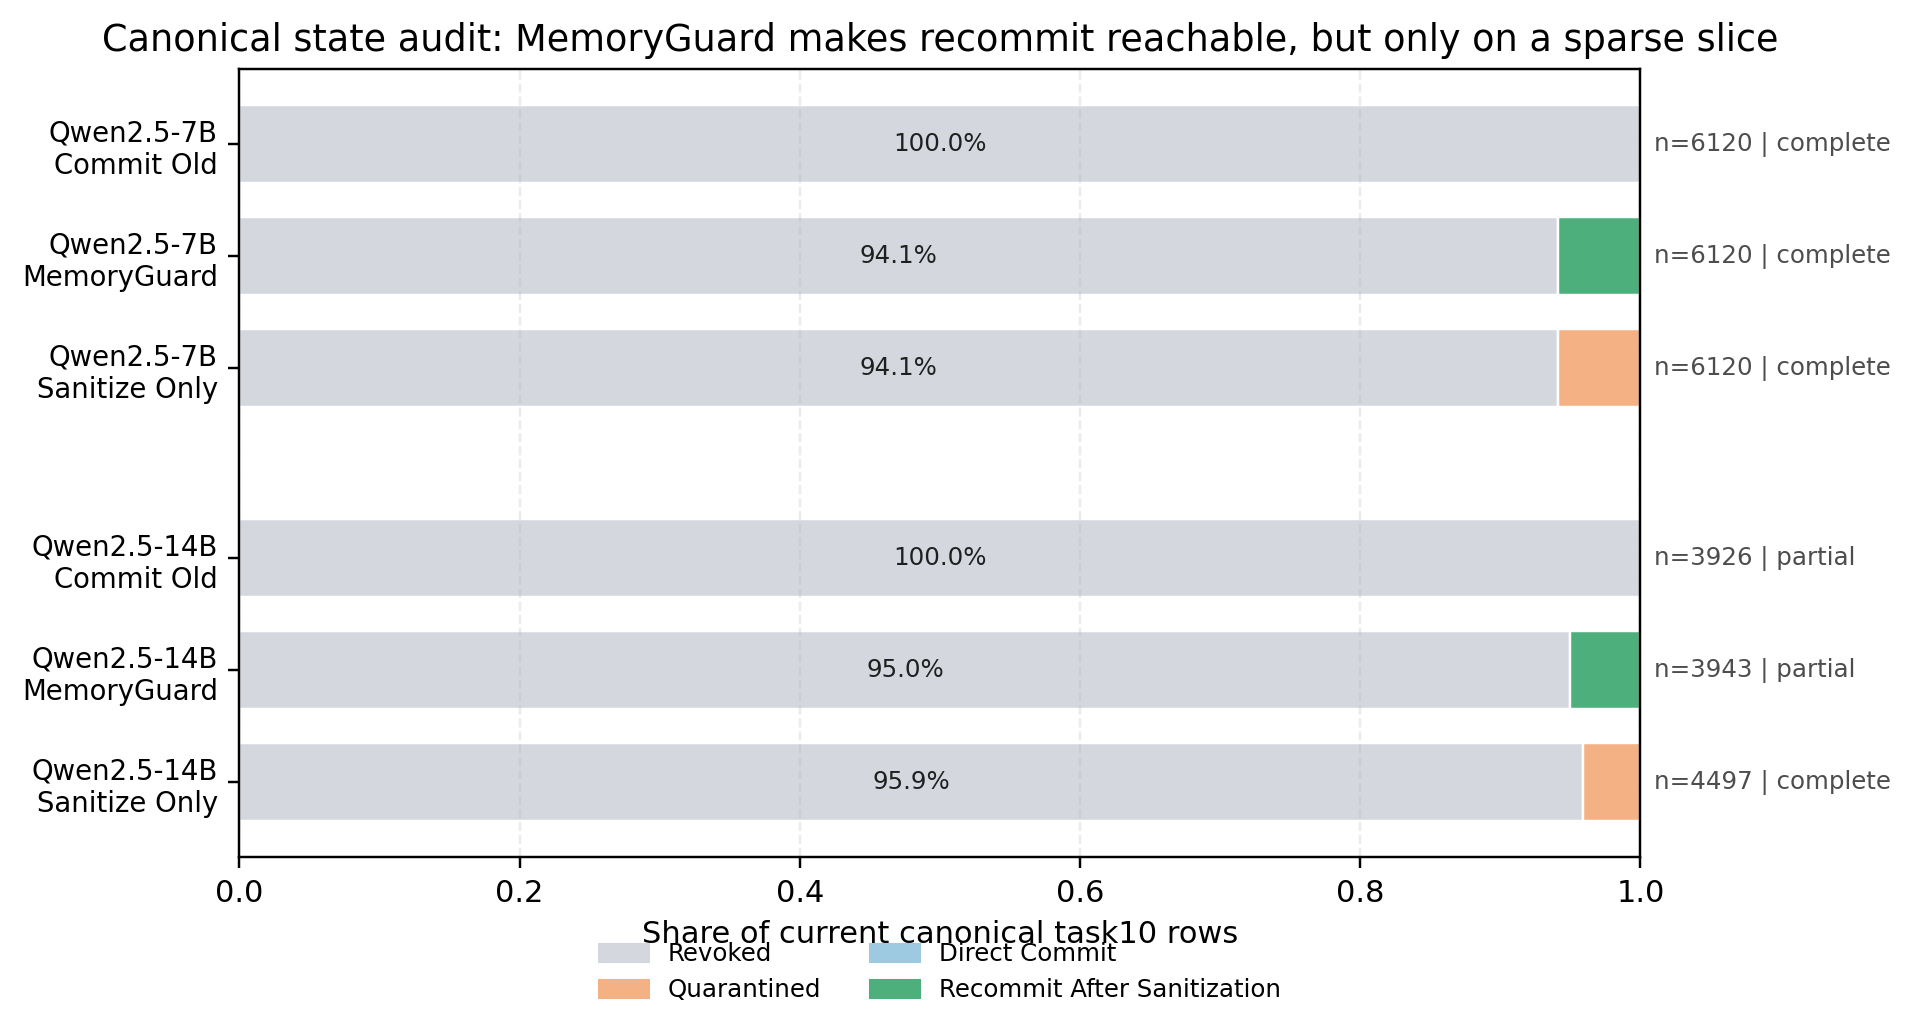
\includegraphics[width=\columnwidth]{figures/memoryguard_state_audit.png}
  \caption{Canonical task10 decision-state audit for the commitment-family
  ablation. The old rule is revoke-only, the repaired rule exposes a
  360-row recommit slice on both Qwen scales, and sanitize-only routes the
  same slice into quarantine instead of reuse.}
  \label{fig:state-audit}
\end{figure}

\paragraph{Sanitize-only proves recommit is a distinct control decision.}
The sanitize-only ablation keeps poison detection and workflow cleaning but
removes the final recommit step. Its zero recommit count on both scales rules
out the easy interpretation that recommit is merely a bookkeeping artifact of
sanitization.

\paragraph{Hybrid counterfactual recommit is the safer canonical
commitment-family variant.}
\texttt{commit\_cfguard} keeps the same 360-row recommit branch as
\texttt{commit\_repair}, but improves the 7B original-task rate from 79.71\%
to 80.39\% and matches the 14B commitment-family ceiling at 86.27\%. On the
current canonical Qwen anchor, it is therefore the strongest or tied-strongest
commitment-family method while preserving zero attack success.

\paragraph{Within-branch quality explains why recommit helps on one scale and
hurts on the other.}
Figure~\ref{fig:branch-quality} looks inside \texttt{commit\_repair} rather
than across methods. On Qwen2.5-7B, revoked rows retain 4080/5760 original
success (70.8\%), while recommitted rows retain 237/360 (65.8\%). On
Qwen2.5-14B, the pattern reverses: revoked rows retain 4920/5760 (85.4\%),
while recommitted rows retain 360/360 (100.0\%). The aggregate utility effect
therefore depends on both branch quality and branch frequency.

\begin{figure}[t]
  \centering
  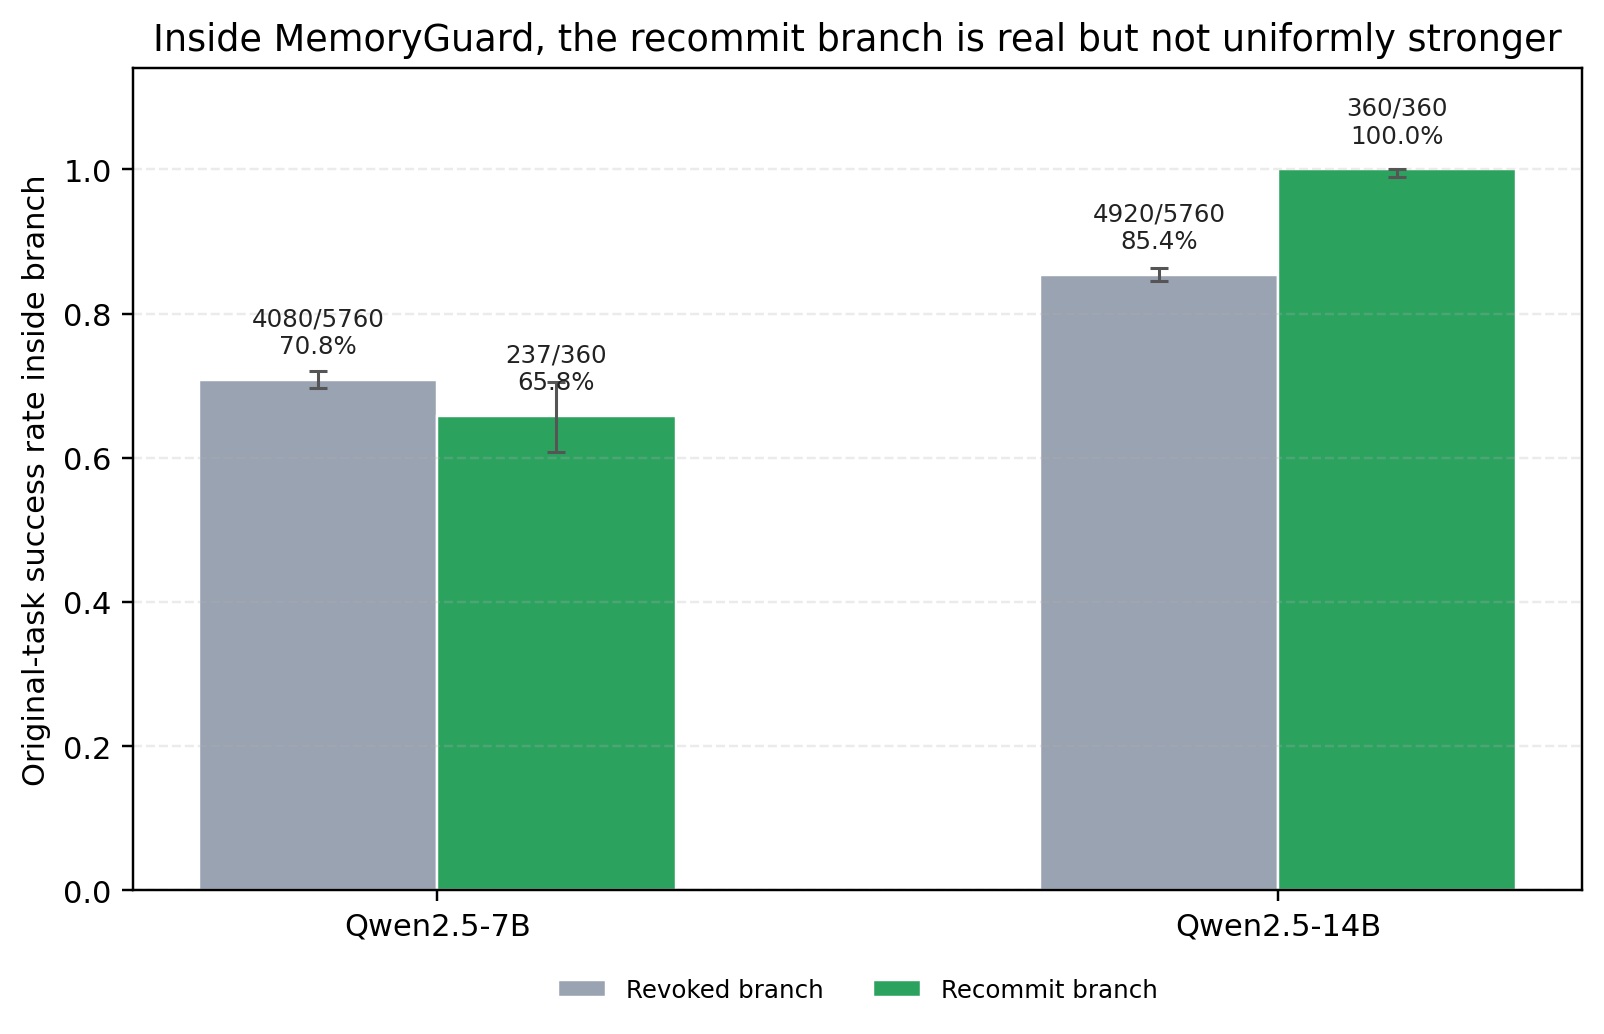
\includegraphics[width=\columnwidth]{figures/memoryguard_recommit_branch_quality.png}
  \caption{Within \texttt{commit\_repair}, original-task success on the
  revoked branch versus the recommit branch. Error bars are 95\% Wilson
  intervals over rows inside each branch. The conditional quality of the
  recommit branch flips across Qwen scales, explaining why recommit is
  aggregate-positive on 7B but not on 14B.}
  \label{fig:branch-quality}
\end{figure}

\paragraph{The overall strongest canonical baseline is still outside the
commitment family.}
\texttt{counterfactual\_guard} remains the best overall canonical method on
both Qwen scales, reaching 94.12\% on 7B and 90.20\% on 14B. Our contribution
is therefore not universal dominance over every defense. It is the repair and
calibration of the commitment family, together with evidence for when a
post-sanitization reuse branch helps, hurts, or needs stronger gating.

\begin{table}[t]
  \caption{Completed support-only Mistral-7B recoverable slice. Each row
  reports the per-seed outcome over the same deterministic 400-row task5
  subset (2 agents $\times$ 5 tasks $\times$ 40 attacker tools); seeds
  \texttt{s0} and \texttt{s1} produce the same rates and are therefore
  summarized together. These rows are used only to probe cross-family
  behavior and are not part of the canonical Qwen claim set.}
  \label{tab:support-smallsample}
  \centering
  \setlength{\tabcolsep}{3.2pt}
  \scriptsize
  \begin{tabular}{llrrrr}
    \toprule
    Model & Method & Cases/Seed & Attack $\downarrow$ & Original $\uparrow$ & Recommit/Seed \\
    \midrule
    \multirow{5}{*}{Mistral-7B}
      & none & 400 & 4.75\% & 0.00\% & 0 \\
      & commit\_old & 400 & \cellcolor{MGGreen}0.00\% & \best{90.00\%} & 0 \\
      & \cellcolor{MGGray}commit\_sanitize\_only & 400 & \cellcolor{MGGreen}0.00\% & \best{90.00\%} & 0 \\
      & \cellcolor{MGBlue}commit\_repair & 400 & \cellcolor{MGGreen}0.00\% & 80.00\% & \cellcolor{MGBlue}\best{120} \\
      & \cellcolor{MGBlue}commit\_cfguard & 400 & \cellcolor{MGGreen}0.00\% & 80.00\% & \cellcolor{MGBlue}\best{120} \\
    \bottomrule
  \end{tabular}
\end{table}


\paragraph{Support-only Mistral recoverable results reinforce the calibration
story.}
Table~\ref{tab:support-smallsample} reports the completed Mistral-7B
recoverable slice. Both completed seeds yield the same rates. The none
baseline leaks on 19/400 cases and never completes the original task.
\texttt{commit\_old} and sanitize-only preserve zero attack success and reach
360/400 original-task success (90.0\%). The recommit-capable variants SCR and
\texttt{commit\_cfguard} also preserve zero attack success and activate
recommit on 120/400 cases, but drop to 320/400 original-task success (80.0\%).
This is the strongest completed
non-Qwen evidence in the current draft, and it argues against any universal
``recommit always helps'' story.

\section{Discussion and Limitations}

The main claim of this paper is narrower than a generic memory-safety story.
On the canonical Qwen anchor, the table is fully closed and safe for ranking,
so we can now say more than ``recommit exists.'' The repaired branch is
reachable, it does not reopen the attack path, and its utility depends on
where and when it is used. That is why the paper is about calibrated reuse
inside the commitment family, not about universal superiority over every
defense.

Recent memory systems and benchmarks emphasize usefulness, persistence, and
long-horizon recall \cite{locomo2024,mem0_2025,amabench2026,memgallery2026},
while recent security work emphasizes attack surfaces, validation, or filtering
\cite{agentdojo2024,amemguard2025,memorygraft2025}. Our evidence sits between
these lines. The important failure is not that commitment-based defense is too
weak on safety, but that it makes the final decision too early. That diagnosis
is supported on canonical Qwen and challenged by the completed Mistral slice,
which is exactly why broader generalization remains open.

This draft has four explicit limitations. First, the headline claim is still
restricted to canonical ASB task10 on Qwen; non-Qwen evidence is currently
limited to one completed Mistral support slice. Second, the repaired reuse
channel remains a reference-only hint rather than direct workflow replay, so
its utility ceiling may be lower than what a stronger executor-side reuse
mechanism could achieve. Third, the defended-run Memory Found field is not a
valid raw-recall metric and cannot be used as retrieval evidence. Fourth, the
current paper does not yet include closed-source or broader model-family
coverage, so cross-family universality remains open.

\paragraph{What still separates this draft from a stronger package.}
The main missing piece is broader support evidence, not more canonical Qwen
closure. Additional DeepSeek and per-agent Mistral diagnostics can sharpen the
scope paragraph and the mechanism explanation, but they are no longer required
to justify the main canonical story. The present version already contains a
closed benchmark table, a state-audit figure, a within-branch quality figure,
and one completed non-Qwen failure case. The next upgrade is better
cross-family evidence, not bigger language.

\section{Related Work}

Long-term memory for LLM agents is now studied from two main angles: utility
and evaluation. System work such as Mem0 and adaptive admission policies asks
how to store and retrieve useful memories efficiently
\cite{mem0_2025,amac2026}. Benchmark work such as LoCoMo, AMA-Bench, and
Mem-Gallery asks whether agents can retain and use information over long
horizons \cite{locomo2024,amabench2026,memgallery2026}. These papers make
long-term memory a first-class capability, but they are not centered on
corrupted memory state or on post-sanitization authority decisions.

A second line of work focuses directly on security. ASB and AgentDojo
formalize prompt injection and related attacks in tool-using agents
\cite{asb2025,agentdojo2024}. Recent memory-specific work studies proactive
memory validation, poisoning, persistent compromise, and extraction attacks
\cite{amemguard2025,mpattack2026,memorygraft2025,mempot2026}. This literature
establishes that memory is a genuine attack surface. What it does not resolve
is the narrower question we study here: once recalled memory has been flagged
and sanitized, should a commitment-based defense still allow bounded reuse?

Our answer is different from both blanket filtering and blanket reuse. SCR is
not a new retrieval system or a new benchmark. It is a repair to a specific
commitment rule. The contribution is the diagnosis that over-revocation comes
from a state-machine decision made too early, together with evidence showing
when a recommit branch is reachable, when it helps, and when it needs stronger
gating.

\section{Conclusion}

We study commitment-based defense for persistent memory poisoning in
tool-augmented agents and identify a deterministic over-revocation failure in
the original state machine. SCR repairs that failure by separating poison
detection from the final commitment decision and recommitting only after
sanitization and alignment checks. The fully closed canonical Qwen task10
table shows that all defended methods preserve zero observed attack success,
the original commitment rule remains revoke-only, and the recommit branch is
real but family-dependent: \texttt{commit\_repair} helps on Qwen2.5-7B and
hurts on Qwen2.5-14B, while \texttt{commit\_cfguard} is the safer
commitment-family compromise on the canonical anchor. The completed
support-only Mistral recoverable slice pushes the same lesson further:
recommit-capable variants preserve security but can still reduce task utility.
The main point is therefore simple. Persistent-memory defense should reason
about whether safe structure survives sanitization and should only reuse that
structure under explicit control. The next step is broader cross-family
validation of that claim, not a broader claim than the current evidence can
support.

\bibliographystyle{ACM-Reference-Format}
\bibliography{refs}

\end{document}
